\chapter{Method Similarity Evaluation}
As discussed in previous chapters, in the context of our research multiple different regression methods operate on common input data. The work shown in this chapter aims to determine to what extent the final models produced by the different regression approaches are similar to one another. We also look into whether the orchestrated hyperparameter tuning approach, discussed in Section \ref{sec:orc_par_tun}, successfully increases this similarity as is intended by design.

The similarity between two linear models is measured with the use of cosine similarity \cite{manning2008introduction}, briefly described in the following section. To determine the overall similarity between two regression methods, we calculate the similarity between their final coefficient vectors for each of the synthetic datasets. Final refers to the models produced by fitting the given regression method on the complete training dataset with the optimal hyperparameter combination obtained from the tuning procedure.


\section{Cosine Similarity}
Cosine similarity measures the similarity between two vectors $A$ and $B$ of equal length $n$. It is defined as shown in Equation \ref{eq:cos_sim} and produces values in the range $[-1,1]$. We used the implementation provided by Scikit-Learn through the cosine\_similarity function.
\begin{equation} \label{eq:cos_sim}
similarity = cos(\theta) = \frac{A \cdot B}{||A||_2||B||_2} = \frac{\sum_{i=1}^{n}A_iB_i}{\sqrt{\sum_{i=1}^{n}A_i^2}\sqrt{\sum_{i=1}^{n}B_i^2}}
\end{equation}


\section{Similarity for CV-MSE tuning} \label{sec:sim_cvmse}
Results from the regression method similarity analysis for all synthetic datasets and use of CV-MSE hyperparameter tuning is shown in Table \ref{tab:sim_cvmse} and Figure \ref{fig:sim_cvmse}. The following observations can be made from the obtained results:

\begin{itemize}
	\item The Lasso and Elastic Net methods produce very similar models. This is to be expected given that the parameter tuning of the Elastic Net commonly selects high values for the L1 ratio(Figure \ref{fig:tun_enet}). As a result, the L1 penalty is a major component of the total Elastic Net penalty.
	\item The GBLasso and Linf methods also show high similarity, which is unsurprising as the Linf method is derived from the GBLasso (see  \ref{sec:linf}).
	\item Our initial expectation was for the TTLP and LTLP methods to be very similar. Surprisingly, the LTLP method bears a stronger similarity to the Lasso and Elastic Net due to its use of the L1 penalty.
\end{itemize}

\begin{sidewaystable}[ph!]
	\begin{center}
		\caption{CV-MSE tuning regression method similarities}
		\label{tab:sim_cvmse}
		\pgfplotstabletypeset[
		multicolumn names,
		col sep=comma,
		header=has colnames,
		columns={Method,Lasso,ENet,Grace,aGrace,GBLasso,Linf,aLinf,TTLP,LTLP,Composite},
		display columns/0/.style={string type, column type = {l}},
		display columns/1/.style={column type={S}, string type, column type = {c}},
		display columns/2/.style={column type={S}, string type, column type = {c}},
		display columns/3/.style={column type={S}, string type, column type = {c}},
		display columns/4/.style={column type={S}, string type, column type = {c}},
		display columns/5/.style={column type={S}, string type, column type = {c}},
		display columns/6/.style={column type={S}, string type, column type = {c}},
		display columns/7/.style={column type={S}, string type, column type = {c}},
		display columns/8/.style={column type={S}, string type, column type = {c}},
		display columns/9/.style={column type={S}, string type, column type = {c}},
		display columns/10/.style={column type={S}, string type, column type = {c}},
		display columns/11/.style={column type={S}, string type, column type = {c}},
		every head row/.style={
			before row={\toprule}, 
			after row/.add={}{
				\arraybackslash
				&$(\sigma_{Lasso})$&$(\sigma_{ENet})$&$(\sigma_{Grace})$&$(\sigma_{aGrace})$&($\sigma_{GBLasso})$&$(\sigma_{Linf})$&$(\sigma_{aLinf})$&$(\sigma_{TTLP})$&$(\sigma_{LTLP})$&$(\sigma_{Composite})$\\
				\midrule\midrule
			}
		},
		every last row/.style={
			after row=\bottomrule
		},
		every nth row={2}{before row=\midrule},
		]{tables/similarity_cvmse.csv}
	\end{center}
\end{sidewaystable}

\begin{figure}[H]
	\centering
	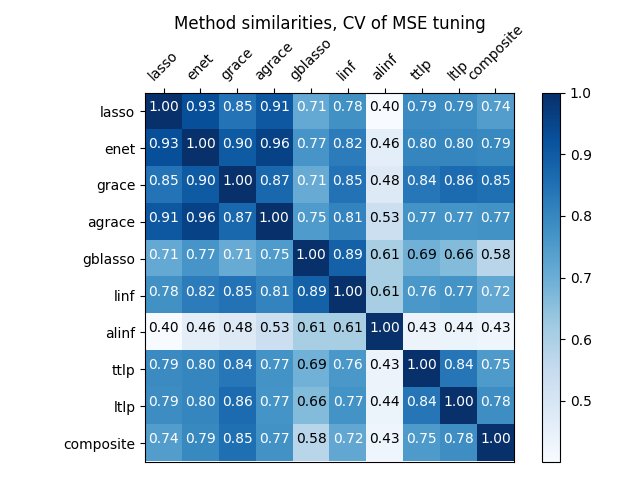
\includegraphics[scale=0.9]{cv_mse_similarities}
	\caption{CV-MSE tuning mean regression method similarities}
	\label{fig:sim_cvmse}
\end{figure}


\section{Similarity for Orchestrated tuning} \label{sec:sim_orctun}
Results from the regression method similarity analysis for all synthetic datasets and use of orchestrated hyperparameter tuning is shown in Table \ref{tab:sim_orctun} and Figure \ref{fig:sim_orctun}.

\begin{table}[H]
	\begin{center}
		\caption{Orchestrated tuning regression method similarities}
		\label{tab:sim_orctun}
		\pgfplotstabletypeset[
		multicolumn names,
		col sep=comma,
		header=has colnames,
		columns={Method,Lasso,ENet,Grace,GBLasso,Linf},
		display columns/0/.style={string type, column type = {l}},
		display columns/1/.style={column type={S}, string type, column type = {c}},
		display columns/2/.style={column type={S}, string type, column type = {c}},
		display columns/3/.style={column type={S}, string type, column type = {c}},
		display columns/4/.style={column type={S}, string type, column type = {c}},
		display columns/5/.style={column type={S}, string type, column type = {c}},
		%display columns/6/.style={column type={S}, string type, column type = {c}},
		every head row/.style={
			before row={\toprule}, 
			after row/.add={}{
				\arraybackslash
				&$(\sigma_{Lasso})$&$(\sigma_{ENet})$&$(\sigma_{Grace})$&($\sigma_{GBLasso})$&$(\sigma_{Linf})$\\
				\midrule\midrule
			}
		},
		every last row/.style={
			after row=\bottomrule
		},
		every nth row={2}{before row=\midrule},
		]{tables/similarity_orctun.csv}
	\end{center}
\end{table}

\begin{figure}[H]
	\centering
	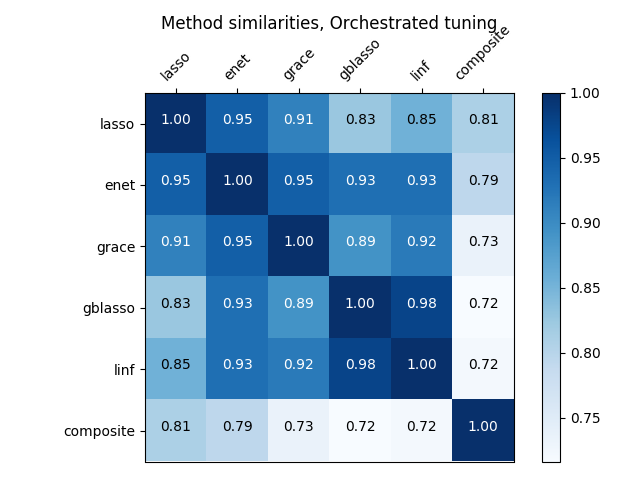
\includegraphics[scale=0.9]{orchestrated_similarities}
	\caption{Orchestrated tuning mean regression method similarities}
	\label{fig:sim_orctun}
\end{figure}


\section{Similarity comparison by tuning method}
The regression method similarities discussed in sections \ref{sec:sim_cvmse} and \ref{sec:sim_orctun} have been merged for easier comparison 
\begin{table}[H]
	\begin{center}
		\caption{Comparison of regression method similarities by tuning method}
		\label{tab:sim_comp}
		\pgfplotstabletypeset[
		multicolumn names,
		col sep=comma,
		header=has colnames,
		columns={Method,Tuning,Lasso,ENet,Grace,GBLasso,Linf,Composite},
		display columns/0/.style={string type, column type = {l}},
		display columns/1/.style={string type, column type = {l}},
		display columns/2/.style={column type={S}, string type, column type = {r}},
		display columns/3/.style={column type={S}, string type, column type = {r}},
		display columns/4/.style={column type={S}, string type, column type = {r}},
		display columns/5/.style={column type={S}, string type, column type = {r}},
		display columns/6/.style={column type={S}, string type, column type = {r}},
		display columns/7/.style={column type={S}, string type, column type = {r}},
		every head row/.style={
			before row={\toprule}, 
			after row={\midrule\midrule}
		},
		every last row/.style={
			after row=\bottomrule
		},
		every nth row={2}{before row=\midrule},
		]{tables/similarity_comparison.csv}
	\end{center}
\end{table}